\section{Code}
\subsection{Java Locks \& Conditions}

\begin{lstlisting}[style=csharp]
public class WarehouseWithLockCondition implements Warehouse {
	private final Lock monitor;
	private final Condition NonFull;
	private final Condition NonEmpty;
	private final int capacity;
	private int items = 0;

	public WarehouseWithLockCondition(int capacity, boolean fair) {
		this.capacity = capacity;
		this.monitor = new ReentrantLock(fair);
		NonEmpty = monitor.newCondition();
		NonFull = monitor.newCondition();
	}

	@Override
	public void put(int amount) throws InterruptedException {
		monitor.lock();

		try {
			while(items + amount > capacity) {
				NonFull.await();
			}

			items += amount;
			NonEmpty.signalAll();
		} finally {
			monitor.unlock();
		}
	}

	@Override
	public void get(int amount) throws InterruptedException {
		monitor.lock();

		try {
			while(amount > items) {
				NonEmpty.await();
			}
			items -= amount;
			NonFull.signalAll();
		} finally {
			monitor.unlock();
		}
	}
}
\end{lstlisting}

\subsection{Java Monitor}

\begin{lstlisting}[style=csharp]
package aufgabe1;

public class WarehouseWithMonitor implements Warehouse {
	private int capacity;
	private int items;

	public WarehouseWithMonitor(int capacity) {
		this.capacity = capacity;
	}

	@Override
	public synchronized void put(int amount) throws InterruptedException {
		while((items + amount) > capacity) {
			wait();
		}
		this.items += amount;
		notifyAll();
	}

	@Override
	public synchronized void get(int amount) throws InterruptedException {
		while(items < amount) {
			wait();
		}
		items -= amount;
		notifyAll();
	}
}
\end{lstlisting}

\subsection{Java Semaphore}

\begin{lstlisting}[style=csharp]
public class WarehouseWithSemaphore implements Warehouse {
	Semaphore capacity;
	Semaphore items = new Semaphore(0, true);

	public WarehouseWithSemaphore(int capacity, boolean fair) {
		this.capacity = new Semaphore(capacity, fair);
	}

	@Override
	public void put(int amount) throws InterruptedException {
		capacity.acquire(amount); // remove from capacity
		items.release(amount); // add items

	}

	@Override
	public void get(int amount) throws InterruptedException {
		items.acquire(amount);
		capacity.release(amount);
	}
}
\end{lstlisting}

\subsection{Rekursiver Thread Pool}

\begin{lstlisting}[style=csharp]
// How to launch
int[] array = new int[] {1,2,3,4,5,6,7,8,9,10};

ForkJoinPool threadPool = new ForkJoinPool();
threadPool.invoke(
		new PairwiseSum(array, 0, array.length / 2));

class PairwiseSum extends RecursiveAction {
    private final int[] array;
    private final int lower, upper;
    private static final int THRESHOLD = 1; // configurable

    public PairwiseSum(int[] array, int lower, int upper) { 
    	this.array = array;
        this.lower = lower;
        this.upper = upper;
    }

    @Override
    protected void compute() {
        if (upper - lower > THRESHOLD) {
            int middle = (lower + upper) / 2;
            invokeAll(
                    new PairwiseSum(array, lower, middle),
                    new PairwiseSum(array, middle, upper)
            );

        } else {
            for (int i = lower; i < upper; i++) {
                array[2 * i] += array[2 * i + 1]; 
                array[2 * i + 1] = 0;
            }
        }
    }
}
\end{lstlisting}

\subsection{Java Async Task}

\begin{lstlisting}[style=csharp]
public class WebDownload {
	public CompletableFuture<String> asyncDownloadUrl(String link) {
		return CompletableFuture.supplyAsync(() -> {
				do_something_dangerous();
				return stringBuilder.toString();
			}
		});
	}
}

\end{lstlisting}

\subsection{Java GUI Thread}

\begin{lstlisting}[style=csharp]
		startButton.addActionListener(event -> {
			// Async function
			CompletableFuture.runAsync(() -> {
				String result = theSupercomputer.calculateUltimateAnswer();
				
				// Invoke when operation is complete
				SwingUtilities.invokeLater(() -> resultLabel.setText("Result: " + result));
			});
		});
\end{lstlisting}

\subsection{.NET Parallel}

\begin{lstlisting}[style=csharp]
Parallel.For(0, array.GetLength(0), row => { 
	Parallel.For(0, array.GetLength(1), col => {
       array[row][col] = (row + 1) * (col + 1);
     }
});

Parallel.Invoke(
    () => RepeatAsync("Test", 10000),
    () => RepeatAsync("Quit", 10000)
);
\end{lstlisting}

\subsection{UI C\#}
\begin{lstlisting}[style=csharp]
async Task downloadAsync(List<Uri> links, Stream output) { 
var client = new HttpClient();
	foreach (Uri uri in links) {
		statusLabel.Content = "Downloading " + uri; 
		if (cancelBox.Checked) {
        	statusLabel.Content = "Cancelled!";
			return; 
		}
		
       	var response = await client.GetAsync(uri);
       	await response.Content.CopyToAsync(output);
     }
     statusLabel.Content = "All done!";
   }
\end{lstlisting}

\subsection{CUDA}
Addieren der Nachbarstellen in einem Array.
\begin{lstlisting}[style=csharp]
__global__ void convolve(int* input, int* output, int length) {
	int i = blockIdx.x * blockDim.x + threadIdx.x;
    if (i < length) {
		int left = i > 0 ? input[i – 1] : 0;
		int right = i < length – 1 ? input[i + 1] : 0; 
		output[i] = left + input[i] + right;
	}
}
\end{lstlisting}

\subsection{Matrix Transposition}
\begin{lstlisting}[style=csharp]
__global__ void transpose(int* matrix, int nofRows, int cols, int* result) {
	int row = blockIdx.x * blockDim.x + threadIdx.x;
	int col = blockIdx.y * blockDim.y + threadIdx.y;
	if (row < rows && col < cols) {
       result[col * rows + row] = matrix[row * cols + col];
     }
}
\end{lstlisting}

\subsection{Completable Future}
\centering
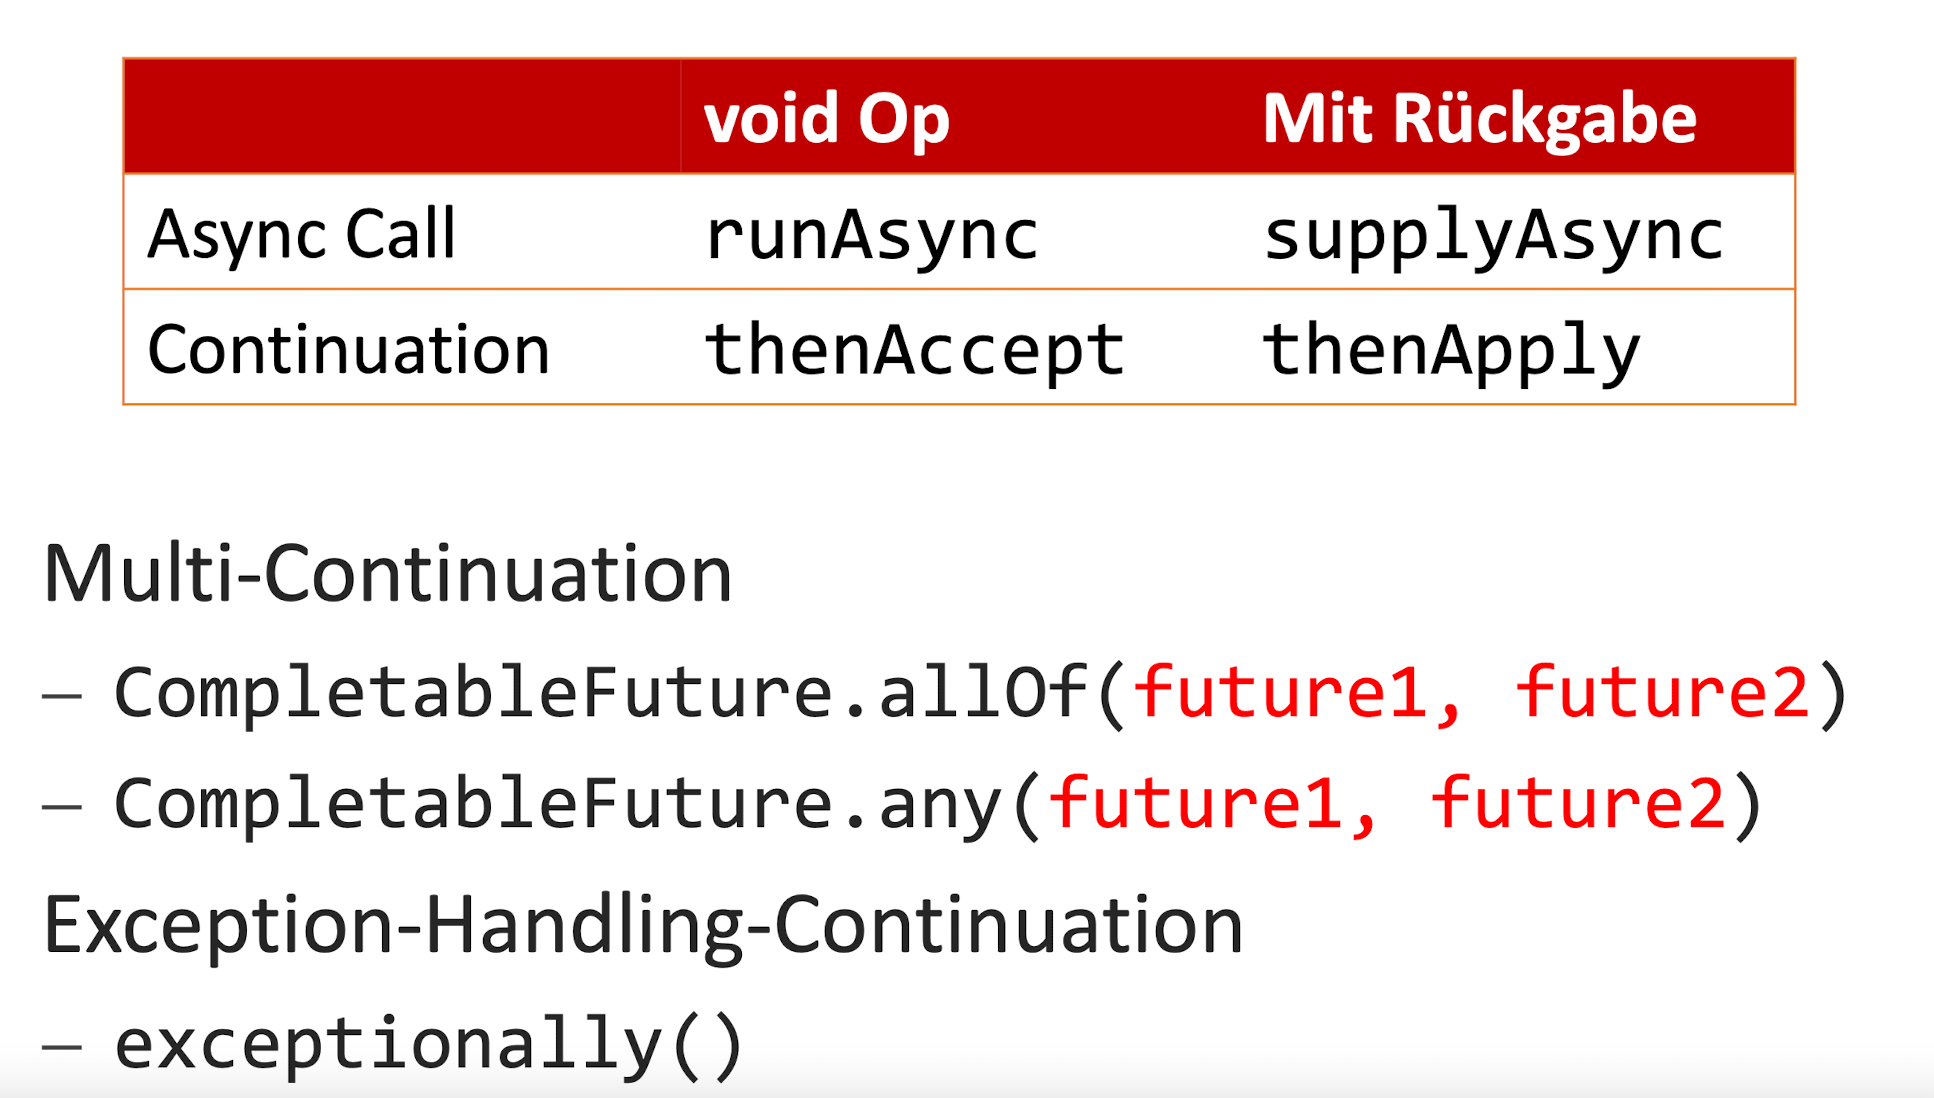
\includegraphics[width=0.75\linewidth]{completablefuture.png}
